\documentclass{article}
\usepackage{tikz}
\usepackage{caption}
\usepackage{subcaption}

\begin{document}

\begin{figure}[h]
    \centering
    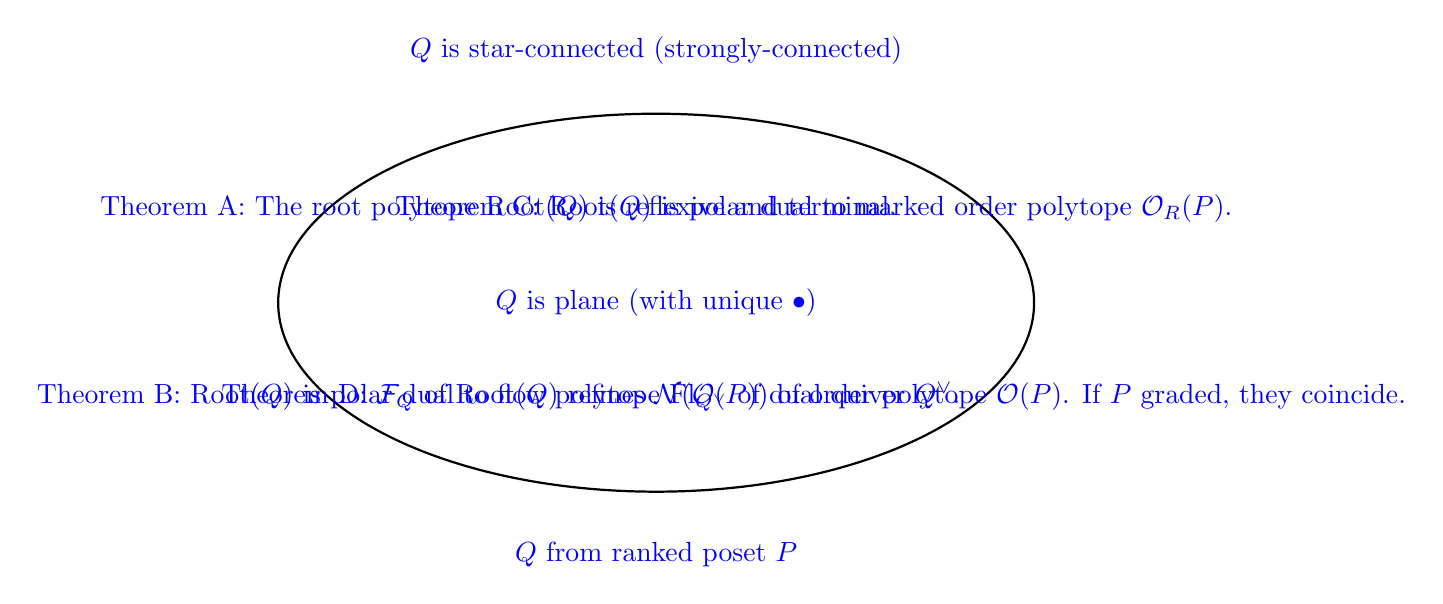
\begin{tikzpicture}[scale=0.8]
        % Draw the main ellipse
        \draw[thick] (0,0) ellipse (6cm and 3cm);
        
        % Text inside the ellipse
        \node at (-2.5,1.5) {\textcolor{blue}{Theorem A: The root polytope $\mathrm{Root}(Q)$ is reflexive and terminal.}};
        \node at (2.5,1.5) {\textcolor{blue}{Theorem C: Root$(Q)$ is polar dual to marked order polytope $\mathcal{O}_R(P)$.}};
        \node at (-2.5,-1.5) {\textcolor{blue}{Theorem B: $\mathrm{Root}(Q)$ is polar dual to flow polytope $\mathrm{Fl}_{Q^\vee}$ of dual quiver $Q^\vee$.}};
        \node at (2.5,-1.5) {\textcolor{blue}{Theorem D: $\mathcal{F}_Q$ of $\mathrm{Root}(Q)$ refines $\mathcal{N}(\mathcal{O}(P))$ of order polytope $\mathcal{O}(P)$. If $P$ graded, they coincide.}};
        
        % Text above the ellipse
        \node at (0,4) {\textcolor{blue}{$Q$ is star-connected (strongly-connected)}};
        
        % Text below the ellipse
        \node at (0,-4) {\textcolor{blue}{$Q$ from ranked poset $P$}};
        
        % Text in the middle
        \node at (0,0) {\textcolor{blue}{$Q$ is plane (with unique $\bullet$)}};
    \end{tikzpicture}
    \caption{Overview of our main results: they appear as \cref{cor:reflexive}, \cref{thm:dual}, \cref{prop:NPreflexive}, \cref{thm:refine}.}
    \label{fig:main_results}
\end{figure}

\end{document}